\documentclass[12pt]{article}

\RequirePackage{amsmath}
\RequirePackage{amsthm}
\RequirePackage{amssymb}
\RequirePackage[mathscr]{eucal}
\RequirePackage{mathtools}
\RequirePackage{etoolbox}

\usepackage{listofitems}

\usepackage[red]{zhoucx-notation}

% correct bad hyphenation here
\hyphenation{op-tical net-works semi-conduc-tor}

\renewcommand{\qedsymbol}{\hfill\rule{2mm}{2mm}}

\pagestyle{fancy}
\fancyhf{}
\setlength{\headheight}{15pt}
\rhead{\textsf{Chapter 20, Neural Networks}}
\lhead{\textsf{Chenxi Zhou}}
\renewcommand{\headrulewidth}{1pt}
\cfoot{\thepage}

\newcommand{\titlebox}[4]{
\begin{tcolorbox}[colback = blue!5!white!95, colframe = blue!70!black
% colback = yellow!30!white, colframe = yellow!70!black 
]
  \noindent \textbf{ #1 } \hfill \textit{#2} 
  \begin{center}
  	 \LARGE{\textbf{#3}}
  \end{center}
\textbf{Chapter:} \textit{#4} \hfill \textbf{Prepared by:} \textit{Chenxi Zhou}
\end{tcolorbox}
}

\tikzset{>=latex} % for LaTeX arrow head
\colorlet{myred}{red!80!black}
\colorlet{myblue}{blue!80!black}
\colorlet{mygreen}{green!60!black}
\colorlet{mydarkred}{myred!40!black}
\colorlet{mydarkblue}{myblue!40!black}
\colorlet{mydarkgreen}{mygreen!40!black}
\tikzstyle{node}=[very thick,circle,draw=myblue,minimum size=22,inner sep=0.5,outer sep=0.6]
\tikzstyle{connect}=[->,thick,mydarkblue,shorten >=1]
\tikzset{ % node styles, numbered for easy mapping with \nstyle
  node 1/.style={node,mydarkgreen,draw=mygreen,fill=mygreen!25},
  node 2/.style={node,mydarkblue,draw=myblue,fill=myblue!20},
  node 3/.style={node,mydarkred,draw=myred,fill=myred!20},
}
\def\nstyle{int(\lay<\Nnodlen?min(2,\lay):3)} % map layer number onto 1, 2, or 3

\begin{document}

\titlebox{Notes on Statistical and Machine Learning}{}{Neural Networks}{20}
\thispagestyle{plain}

\vspace{10pt}

This note is prepared based on \textit{Chapter 11, Neural Networks} in \textcite{Friedman2001-np}. 


\section*{I. Neural Networks}

\begin{enumerate}[label=\textbf{\arabic*.}]

	\item \textbf{Main Idea:} The central idea of the neural networks is to 
	\begin{enumerate}
		\item extract linear combinations of the input variables as \emph{derived features}, and 
		\item model the target as a \emph{non-linear} function of these derived features. 
	\end{enumerate}
	
	\item \textbf{Basics:} In this section, we discuss the ``vanilla'' neural network, also called the \textit{single hidden layer back-propagation network} or \textit{single layer perceptron}. 
	
	In this sense, a neural network is a \emph{two-stage regression} or \emph{classification model} represented by a network diagram (see Figure \ref{network.diagram}). From a statistical perspective, they are just nonlinear statistical models. 
	
	\begin{figure}[h!]
		\centering 
		% NEURAL NETWORK
		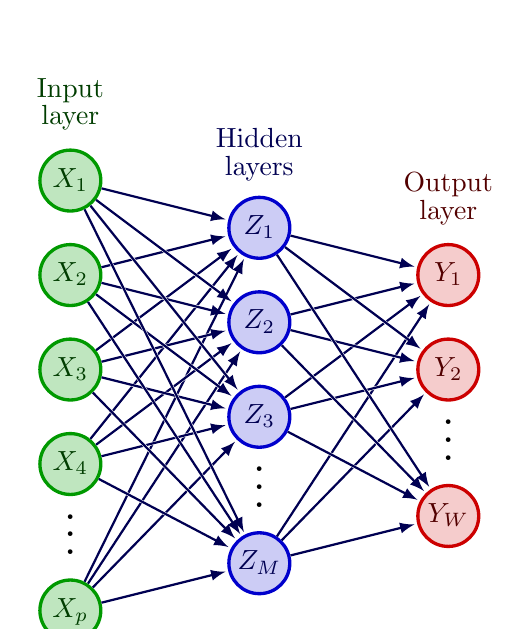
\begin{tikzpicture}[x=2.4cm,y=1.2cm]
			\readlist\Nnod{5,4,3} % array of number of nodes per layer
			\readlist\Nstr{p,M,W} % array of string number of nodes per layer
			\readlist\Cstr{X,Z,Y} % array of coefficient symbol per layer
			\def\yshift{0.55} % shift last node for dots
			
			% LOOP over LAYERS
			\foreachitem \N \in \Nnod{
				\def\lay{\Ncnt} % alias of index of current layer
				\pgfmathsetmacro\prev{int(\Ncnt-1)} % number of previous layer
				\foreach \i [evaluate={\c=int(\i==\N); \y=\N/2-\i-\c*\yshift;
				\x=\lay; \n=\nstyle;
				\index=(\i<\N?int(\i):"\Nstr[\n]");}] in {1,...,\N}{ % loop over nodes
				% NODES
				\node[node \n] (N\lay-\i) at (\x,\y) {$\strut\Cstr[\n]_{\index}$
			};
			
			% CONNECTIONS
			\ifnumcomp{\lay}{>}{1}{ % connect to previous layer
				\foreach \j in {1,...,\Nnod[\prev]}{ % loop over nodes in previous layer
				\draw[white,line width=1.2,shorten >=1] (N\prev-\j) -- (N\lay-\i);
				\draw[connect] (N\prev-\j) -- (N\lay-\i);
			}
			
			\ifnum \lay=\Nnodlen
			%\draw[connect] (N\lay-\i) --++ (0.5,0); % arrows out
			\fi }
%			{\draw[connect] (0.5,\y) -- (N\lay-\i); % arrows in}
			}
			\path (N\lay-\N) --++ (0,1+\yshift) node[midway,scale=1.6] {$\vdots$}; % dots
			}
			
			% LABELS
			\node[above=3,align=center,mydarkgreen] at (N1-1.90) {Input\\[-0.2em]layer};
			\node[above=2,align=center,mydarkblue] at (N2-1.90) {Hidden\\[-0.2em]layers};
			\node[above=3,align=center,mydarkred] at (N\Nnodlen-1.90) {Output\\[-0.2em]layer};
		\end{tikzpicture}
		
		\caption{Schematic of a single hidden layer, feed-forward neural network. }
		\label{network.diagram}
		
	\end{figure}
	
	\begin{enumerate}
		\item \textit{Output Layer:} We use $W$ to denote the number of units in the output layer. 
		\begin{itemize}
			\item For regression, typically $W = 1$ and there is only one output unit $Y_1$. It can be extended to handle multiple quantitative responses. 
			\item For $W$-class classification, there are $W$ units at the output layer with the $w$-th unit modeling the probability of Class $w$. There are $W$ target measurements $Y_w$, for all $w = 1, \cdots, W$, each being coded as a binary variable for the $w$-th class. 
		\end{itemize}
		
		\item \textit{Derived features:} Derived features $\sets{Z_m}_{m=1}^M$ are created from linear combinations of the inputs $X_1, \cdots, X_p$, and then the target $Y_k$ is modeled as a function of linear combinations of the $Z_m$'s, that is, 
		\begin{equation*}
			\begin{aligned}
				& \, Z_m = \sigma \parens{\alpha_{0,m} + \balpha_{m}^\top X}, \qquad \qquad && \, m = 1, \cdots, M, \\ 
				& \, T_w = \beta_{0,w} + \bbeta_w^\top Z, && \, w = 1, \cdots, W, \\ 
				& \, Y_w = f_w \parens{X} = g_w \parens{T}, && \, w = 1, \cdots, W, 
			\end{aligned}
		\end{equation*}
		where $Z = \parens{Z_1, Z_2, \cdots, Z_M}$ and $T = \parens{T_1, T_2, \cdots, T_W}$. 
		
		\item \textit{Hidden Layer:} The units in the middle of the network, computing the derived features $Z_m$, are called \textit{hidden units} because $Z_m$ are \emph{not} directly observed. 
		
		\textit{Remark.} In general, there can be more than one hidden layer. We can think of the $Z_m$ as a basis expansion of the original inputs $X$. 
		
		\item \textit{Activation Function:} The activation function $\sigma$ is usually chosen to be the sigmoid $\sigma \parens{v} = 1/ \parens{1 + e^{-v}}$. By using a nonlinear transformation $\sigma$, it greatly enlarges the class of linear models. 
		
		\textit{Remark.} If $\sigma$ is the identity function, then the entire model collapses to a linear model in the input variables. Hence, a neural network can be thought of as a nonlinear generalization of the linear model, both for regression and classification. 
		
		\item \textit{Output Function:} The output function $\sets{g_w}_{w=1}^W$ allows a final transformation of the vector of outputs $T$. 
		\begin{itemize}
			\item For regression, we typically choose the identity function $g_w \parens{T} = T_w$ for all $w = 1, 2, \cdots, W$; 
			\item For classification, one popular choice is the softmax function 
			\begin{align}
				g_w \parens{T} = \frac{e^{T_w}}{\sum_{\ell=1}^W e^{T_{\ell}}}, \qquad \text{ for all } w = 1, 2, \cdots, W. 
			\end{align}
		\end{itemize}
		
	\end{enumerate}
	
	\item \textbf{Connection between Neural Network and Projection Pursuit Regression:} Neural networks with one hidden layer has exactly the same form as the projection pursuit model. The only difference is that the PPR model uses nonparametric functions $g_m$, while the neural network uses $\sigma$. 
	
	Viewing the neural network model as a PPR model, we have 
	\begin{align}
		g_m \parens{\bome_m^\top X} = & \, \beta_m \sigma \parens{\alpha_{0,m} + \balpha_m^\top X} \nonumber \\ 
		= & \, \beta_m \sigma \parens{\alpha_{0,m} + \norm{\balpha_m}_2 \parens{\bome_m^\top X}}, 
	\end{align}
	where $\bome_m := \balpha_m / \norm{\balpha_m}_2$ is the $m$-th unit vector. 

\end{enumerate}


\section*{II. Fitting Neural Networks}

\begin{enumerate}[label=\textbf{\arabic*.}]

	\item \textbf{Weights:} The unknown parameters in neural networks are often called \textit{weights}. In a neural network with one hidden layer, denote the complete set of weights by $\btheta$, consisting of 
	\begin{enumerate}
		\item $\sets{\alpha_{0,m}, \balpha_m \,\vert\, \balpha_m \in \Real^p}_{m = 1, \cdots, M}$, which are $M \parens{p+1}$ parameters, 
		\item $\sets{\beta_{0,w}, \bbeta_w \,\vert\, \bbeta_w \in \Real^M}_{w = 1, \cdots, W}$, which are $W \parens{M+1}$ parameters. 
	\end{enumerate}
	
	\item \textbf{Loss Function:} 
	\begin{enumerate}
		\item For regression, we use sum-of-squared errors as the loss function 
		\begin{align}
			L \parens{\btheta} = \sum_{w=1}^W \sum_{i=1}^n \parens{y_{i,w} - f_w \parens{\bx_i}}^2. 
		\end{align}
		\item For classification, use either squared error or cross-entropy  
		\begin{align}
			L \parens{\btheta} = - \sum_{w=1}^W \sum_{i=1}^n y_{i,w} \log f_w \parens{\bx_i}, 
		\end{align}
		and the corresponding classifier is $G \parens{\bx} = \argmax_{w=1,\cdots,W} f_w \parens{\bx}$. 
	\end{enumerate}
	
	\item \textbf{Regularization:} Typically, we add a penalty term to $L$ or stop the algorithm early to avoid an overfit solution in fitting a neural network. 
	
	\item \textbf{Minimization Method:} We typically minimize $L$ by gradient descent, called \textit{back-propagation} in this setting. The gradient can be easily derived using the chain rule for differentiation. 
	
	\item \textbf{Back-Propagation Using Squared Error Loss:} Consider the squared error loss. Let $z_{m,i} := \sigma \parens{\alpha_{0,m} + \balpha_m^\top \bx_i}$ and $\bz_i := \parens{z_{1,i}, z_{2,i}, \cdots, z_{M,i}}$. Then, we have 
	\begin{align*}
		L \parens{\btheta} = \sum_{i=1}^n L_i = \sum_{i=1}^n \sum_{w=1}^W \parens{y_{i,w} - f_w \parens{\bx_i}}^2. 
	\end{align*}
	And, 
	\begin{align*}
		\frac{\partial L_i}{\partial \beta_{w,m}} = & \, -2 \parens{y_{i,w} - f_w \parens{\bx_i}} g_w' \parens{\bbeta_w^\top \bz_i} z_{m,i}, \\ 
		\frac{\partial L_i}{\partial \alpha_{m,\ell}} = & \, - \sum_{w=1}^W 2 \parens{y_{i,w} - f_w \parens{\bx_i}} g_w' \parens{\bbeta_w^\top \bz_i} \beta_{w,m} \sigma' \parens{\balpha_m^\top \bx_i} x_{i,\ell}. 
	\end{align*}
	Then, the gradient update at the $\parens{j+1}$-st iteration has the form 
	
	\begin{equation}\label{grad.updates}
		\begin{aligned}
			\beta_{w,m}^{\parens{j+1}} = & \, \beta_{w,m}^{\parens{j}} - \gamma_j \sum_{i=1}^n \frac{\partial L_i}{\partial \beta_{w,m}} \bigg\vert_{\beta_{w,m} = \beta_{w,m}^{\parens{j}}}, \\ 
			\alpha_{m,\ell}^{\parens{j+1}} = & \, \alpha_{m\ell}^{\parens{j}} - \gamma_j \sum_{i=1}^n \frac{\partial L_i}{\partial \alpha_{m,\ell}} \bigg\vert_{\alpha_{m,\ell} = \alpha_{m,\ell}^{\parens{j}}}, 
		\end{aligned}
	\end{equation}
	where $\gamma_j > 0$ is the learning rate. 
	
	If we define 
	\begin{align*}
		\delta_{w,i} := & \, -2 \parens{y_{i,w} - f_w \parens{\bx_i}} g_w' \parens{\bbeta_w^\top \bz_i}, \\ 
		s_{m,i} := & \, - \sum_{w=1}^W 2 \parens{y_{i,w} - f_w \parens{\bx_i}} g_w' \parens{\bbeta_w^\top \bz_i} \beta_{w,m} \sigma' \parens{\balpha_m^\top \bx_i}, 
	\end{align*}
	we can write 
	\begin{align}
		\frac{\partial L_i}{\partial \beta_{w,m}} = \delta_{w,i} z_{m,i}, \qquad \text{ and } \qquad \frac{\partial L_i}{\partial \beta_{m,\ell}} = s_{m,i} x_{i,\ell}. 
	\end{align}
	The quantities $\delta_{w,i}$ and $s_{m,i}$ are ``errors'' from the current model at the output and hidden layer units, respectively. There errors satisfy the equation 
	\begin{align}\label{back.prop}
		s_{m,i} = \sigma' \parens{\balpha_m^\top \bx_i} \sum_{w=1}^W \beta_{w,m} \delta_{w,i}, 
	\end{align}
	known as the \textit{back-propagation equations}. 
	
	\item \textbf{Two-Pass Algorithm:} 
	\begin{enumerate}
		\item \textit{Forward Pass:} current weights are fixed and the predicted values $\hat{f}_w \parens{\bx_i}$ are computed; 
		\item \textit{Backward Pass:} Compute the errors $\delta_{w,i}$ and then use back-propagation equation \eqref{back.prop} to compute errors $s_{m,i}$. 
	\end{enumerate}
	
	\item \textbf{Comments on Back-Propagation and Two-Pass Algorithm:} 
	\begin{enumerate}
		\item \textit{Advantages:} The advantages of back-propagation are its simple, local nature. It can be implemented efficiently on a parallel architecture computer. 
	
		\item \textit{Disadvantages:} Back-propagation can be very slow. Better approaches include conjugate gradients and variable metric methods. 
	\end{enumerate}
	
	\textit{Remark.} Second-order optmization techniques such as Newton's method are \emph{not} attractive in the neural network setting, because the Hessian matrix of $L$ can be very large. 
	
	\item \textbf{Batch Learning and Online Learning:} Updates \eqref{grad.updates} are a kind of \textit{batch learning}, with the parameter updates being a sum over all of the training cases. 

	\textit{Online learning} refers to processing each observation one at a time, updating the gradient after each training case, and cycling through the training cases many times. Online training allows the network to handle very large training sets, and also to update the weights as new observations come in. 
	
	A \textit{training epoch} refers to one sweep through the entire training set. 
	
	\item \textbf{Learning Rate:} 
	\begin{enumerate}
		\item In \textit{batch learning}, the learning rate $\gamma_j$ for is usually taken to be a constant, and can also be optimized by a line search that minimizes the error function at each update; 
		\item In \textit{online learning}, $\gamma_j$ should decrease to zero as the iteration $j \to \infty$. This learning is a form of stochastic approximation. Algorithm is guaranteed to converge if $\gamma_j \to 0$, $\sum_{j=1}^{\infty} \gamma_j = \infty$ and $\sum_{j=1}^{\infty} \gamma^2_j < \infty$. 
	\end{enumerate}
	
\end{enumerate}


\section*{III. Practical Issues in Training Neural Networks}

\begin{enumerate}[label=\textbf{\arabic*.}]

	\item \textbf{Starting Values for Weights:} Usually starting values for weights are chosen to be random values near zero. Hence, the model starts out nearly linear, and becomes nonlinear as the weights increase. 
	
	\item \textbf{Methods to Avoid Overfitting:} 
	\begin{enumerate}
		\item \textit{Early Stopping:} Train the model only for a while and stop well before we approach the global minimum. A validation dataset is useful for determining when to stop. 
		\item \textit{Weight Decay:} Add a penalty to the error function and minimize $L \parens{\btheta} + \lambda J \parens{\btheta}$, where 
		\begin{align}\label{pel1}
			J \parens{\btheta} = \sum_{w,m} \beta_{w,m}^2 + \sum_{m,\ell} \alpha_{m,\ell}^2, 
		\end{align}
		and $\lambda > 0$ is a tuning parameter and can be chosen using the cross validation. Larger values of $\lambda$ will tend to shrink the weights toward zero. 
		
		Other forms for the penalty have been proposed, for example,
		\begin{align}
			J \parens{\btheta} = \sum_{w,m} \frac{\beta_{w,m}^2}{1 + \beta_{w,m}^2} + \sum_{m,\ell} \frac{\alpha_{m,\ell}^2}{1 + \alpha_{m,\ell}^2}, 
		\end{align}
		known as the \textit{weight elimination penalty}. This has the effect of shrinking smaller weights more than \eqref{pel1} does. 
	\end{enumerate}
	
	\item \textbf{Scaling of Inputs:} The scaling of input variables determines the effective scaling of the weights in the bottom layer, and has a large effects on the final output. 
	
	\textit{Recommendation:} At the outset, it is best to standardize all inputs to have mean zero and standard deviation one. 
	
	\item \textbf{Choice of the Number of Hidden Units:} It is usually better to have too many hidden units than too few. 
	\begin{itemize}
		\item With too few hidden units, the model might not have enough flexibility to capture the nonlinearities in the data; 
		\item With too many hidden units, the extra weights can be shrunk toward zero if appropriate regularization is used. 
	\end{itemize}
	Typically choice of the number of hidden units is between 5 and 100. It is most common to put down a reasonably large number of units and train them with regularization. 
	
	\item \textbf{Choice of the Number of Hidden Layers:} Choice of the number of hidden layers is guided by background knowledge and experimentation. Use of multiple hidden layers allows construction of hierarchical features at different levels of resolution. 
	
	\item \textbf{Multiple Local Minima:} The loss function $L$ is non-convex, possessing many local minima. 
	\begin{enumerate}
		\item \textit{Solution 1:} Try a number of random starting configurations, and choose the solution giving lowest (penalized) error. 
		\item \textit{Solution 2:} Use the average predictions over the collection of networks as the final prediction. 
	\end{enumerate}

\end{enumerate}

\printbibliography

\end{document}
